\documentclass[number,preprint,review,12pt]{elsarticle}

%% Basic packages
\usepackage{amssymb}
\usepackage{amsmath}
\usepackage{graphicx}
\usepackage{grffile}
\usepackage{booktabs}
\usepackage{lineno}
\usepackage{float}
\usepackage{hyperref}
\usepackage{doi}

%% Journal setting
\journal{Knowledge-Based Systems}

\begin{document}

\begin{frontmatter}

%% Title
\title{Agri-MetaRL: An Agricultural Meta-Reinforcement Learning Algorithm for Greenhouse Climate Control}

%% Author information
\author[inst1]{Qiang Huang\corref{cor1}\footnotemark[1]}
\ead{13499@sicau.edu.cn}
\cortext[cor1]{Corresponding author}

\author[inst1]{Tianchen Xie\footnotemark[1]}
\ead{2024319025@stu.sicau.edu.cn}

\author[inst1]{Chengkai Yu}
\ead{yck@stu.sicau.edu.cn}

\author[inst1]{Zhaoxiong Ma}
\ead{mazhaoxiong@stu.sicau.edu.cn}

%% Affiliations
\affiliation[inst1]{organization={College of Information Engineering, Sichuan Agricultural University},
            addressline={},
            city={Ya'an},
            postcode={625014},
            country={China}}

\footnotetext[1]{These authors contributed equally to this work.}

%% Abstract
\begin{abstract}
Greenhouse climate control aims to ensure suitable growing conditions and reduce energy consumption. Greenhouse systems exhibit strong nonlinearity, time-varying disturbances, and changing crop stages, which make traditional methods (PID, rule-based control, model predictive control) prone to failure under cross-season and cross-weather conditions. Reinforcement learning (RL) offers a data-driven path, but most studies train a single policy and pay insufficient attention to cross-task transfer. This paper formulates greenhouse control as a set of related tasks defined by weather year, start date, and scenario conditions. It proposes Agri-MetaRL, a meta-reinforcement learning algorithm that improves advantage estimation at the algorithmic level. Based on Recurrent PPO, Agri-MetaRL introduces a support-query advantage correction mechanism and a custom module, MetaAdvantageHead, which encodes task context from support trajectories and performs task-adaptive correction on query trajectories. The design avoids extra policy branches and heavy bi-level optimizers. Experiments on the GreenLight-Gym benchmark under 5 random seeds show that Agri-MetaRL achieved a final mean training return of 3955, higher than Recurrent PPO (3886) and PPO (3811). Under the fixed protocol, Agri-MetaRL had the lowest violation steps for temperature, humidity, and CO$_2$, and the highest EPI of 3.46 €/m$^2$.
\end{abstract}

%% Graphical abstract
\begin{graphicalabstract}
%\includegraphics{figures/graphical_abstract.png}
\end{graphicalabstract}

%% Highlights (each no more than 85 characters)
\begin{highlights}
\item Greenhouse control is modeled as a task distribution over weather and scenario.
\item MetaAdvantageHead on Recurrent PPO for task-adaptive advantage correction.
\item Evaluation protocol with training and held-out testing is constructed.
\item Agri-MetaRL achieves highest EPI (3.46 €/m$^2$) under the current protocol.
\item The method shows competitive temperature control and held-out performance.
\end{highlights}

%% Keywords
\begin{keyword}
Greenhouse climate control \sep Reinforcement learning \sep Meta-reinforcement learning \sep Recurrent PPO \sep Smart agriculture
\end{keyword}

\end{frontmatter}

\linenumbers

\section{Introduction}
Protected agriculture provides stable growing conditions for crops by regulating temperature, humidity, CO$_2$ concentration, and radiation. This approach can increase yield per unit area, extend supply periods, and resist extreme weather~\cite{vanhenten2006greenhouse,li2023smart}. In modern high-tech greenhouses, environmental variables, crop state, and actuators are strongly coupled. External weather and crop growth stages change continuously. Thus, greenhouse control has characteristics of strong time-variation, partial observability, and multi-objective optimization. How to achieve high returns, low energy consumption, and strong generalization control while ensuring crop safety bounds is one of the core problems at the intersection of agricultural engineering and intelligent control.

Traditional greenhouse control often uses PID, threshold rules, and manual experience-based strategies~\cite{berenguel1997temperature,vanstraten2010optimal}. These methods are simple to implement and highly interpretable. But parameters are usually tuned for specific seasons, specific greenhouses, and specific crop stages. When weather distribution changes or crop state shifts, re-tuning is often required. Model predictive control (MPC) can use future predictions and explicit constraints to improve control quality~\cite{camacho2013mpc}. But MPC performance depends on high-precision greenhouse dynamics models and stable solving processes. When model error, parameter uncertainty, and long-horizon rolling optimization coexist, deployment cost remains high. This has been reflected in studies on economic greenhouse MPC and full-cycle crop setpoint optimization~\cite{panagopoulos2025cascaded,garcia2023multi,van2025optimal}. RL-guided MPC and RL-based MPC have been proposed as compromise solutions to balance learning ability and optimization structure~\cite{msaad2025rl,mallick2025reinforcement}.

In recent years, reinforcement learning (RL) has received wide attention. RL does not rely on precise analytical models and can directly optimize policies toward cumulative returns~\cite{sutton2018reinforcement,brockman2016gym,mnih2015dqn,arulkumaran2017brief,lillicrap2015ddpg,haarnoja2018sac,duan2016benchmark}. GreenLight-Gym provides a standardized high-fidelity benchmark environment for greenhouse RL~\cite{van2025greenlight}. Greenhouse RL and deep RL control have been used in recent years for comparing RL with MPC, improving energy efficiency, and introducing interactive control~\cite{morcego2023reinforcement,ajagekar2023energy,xiao2026grower}. But most existing work limits training to a single or nearly single environment distribution. As a result, the learned policies are often closer to ``a strong controller trained on one representative task'' than to ``a task-aware update structure that transfers across a family of related tasks.''

From a learning perspective, changes in weather year, start planting date, parameter perturbations, and scenario coefficients make greenhouse control better viewed as a family of related tasks rather than a single MDP. The goal of meta-reinforcement learning (Meta-RL) is not only to learn a static optimal policy, but also to learn an update structure that transfers across related tasks~\cite{finn2017maml,duan2016rl2,wang2020survey,ravi2017optimization}. Meta-gradient RL, distributional meta-gradient RL, first-order meta-learning, and comparisons of fine-tuning with Meta-RL all show that learning update rules or adaptation priors can significantly affect cross-task performance~\cite{xu2020meta,yin2023distributional,zhao2022effectiveness,nichol2018reptile}. Inspired by this line of work, this paper proposes a new meta-reinforcement learning algorithm, Agri-MetaRL, and formulates greenhouse control as a Meta-RL problem over weather year, start date, and scenario conditions. The contribution of this paper lies in algorithm design, not merely in applying off-the-shelf RL to greenhouse scenarios. Instead of adding multi-policy branches or constructing heavy inner-outer optimizers, this paper performs task-adaptive correction on advantage estimation. Specifically, task context is extracted from support trajectories, and corrected advantages are generated on query trajectories to guide PPO policy updates. This design aligns with the research thread of improving RL algorithms by learning optimization objectives or update rules~\cite{lu2022discovered,oh2025discovering}.

Unlike the traditional ``single-environment RL + test-period extrapolation,'' this paper introduces a task-partitioned training skeleton at the implementation level. Each task segment in the training buffer is split into support and query sets~\cite{vinyals2016matching,snell2017prototypical,rakelly2019pearl}. The support set encodes context. The query set computes task-adaptive advantages for the auxiliary correction module. This design brings Agri-MetaRL closer to task-conditioned policy optimization while retaining training-flow compatibility with standard PPO and engineering simplicity.

The main contributions of this paper are as follows:
\begin{enumerate}
    \item For greenhouse climate control, a task-distribution modeling approach over weather year, start date, and scenario conditions is proposed, together with corresponding training and testing protocols for agricultural meta-reinforcement learning.
    \item A new meta-RL algorithm design is proposed: task-adaptive correction is introduced at the advantage estimation step, rather than merely applying off-the-shelf RL to greenhouse scenarios.
    \item The custom module MetaAdvantageHead is designed and implemented. It performs lightweight task-conditioned advantage correction through support-set context encoding. This module differs from standard Recurrent PPO and is a researcher-developed algorithm component.
    \item On the GreenLight-Gym benchmark, a unified evaluation matrix is constructed including learning curves, climate bounds, economic metrics, and held-out evaluation.
\end{enumerate}

\section{Materials and Methods}
\subsection{Simulation Environment}
Experiments in this paper were conducted on the GreenLight-Gym greenhouse reinforcement learning platform~\cite{van2025greenlight,vanhenten2006greenhouse,taksen2024gymnasium}. The platform exposes high-fidelity greenhouse climate dynamics, crop growth, and actuator control through the Gymnasium interface. It supports flexible configuration of weather, parameters, and observation modules. The simulation object is a Venlo-type glass greenhouse common in the Netherlands, with tomato (\textit{Solanum lycopersicum}) as the crop. External weather uses Amsterdam historical weather data. Each episode represents a 60 d growth window. The control step is 15 min. Thus each episode contains 5760 control steps.

\subsection{Observation and Action Spaces}
The agent's observation vector has 263 dimensions. It consists of six types of information, as shown in Table~\ref{tab:state_space}.

\begin{table}[H]
\centering
\caption{Composition of the agent observation vector in the GreenLight-Gym tomato greenhouse environment}
\label{tab:state_space}
\begin{tabular}{lc}
\toprule
Component module & Dimension \\
\midrule
Indoor climate & 4 \\
Crop state & 3 \\
Control signals & 6 \\
Current weather & 5 \\
Time encoding & 5 \\
Weather forecast & 240 \\
\bottomrule
\end{tabular}
\end{table}

Observations include indoor climate, crop state, current control inputs, current weather, time encoding, and weather forecasts for the next 48 time steps. Running mean and variance were used to normalize observations during training. The action space is a 6-dimensional continuous vector. It corresponds to six actuator types: heating, CO$_2$ injection, thermal screen, ventilation, supplemental lighting, and shade screen. The action range is $[-1, 1]$. The system updates control inputs in an incremental manner:
\begin{equation}
u_{t+1} = \mathrm{clip}(u_t + a_t \cdot \Delta u_{\max}, u_{\min}, u_{\max}),
\end{equation}
where $\Delta u_{\max}=0.1$. The incremental control mechanism can reduce abrupt actuator changes and improve control smoothness and training stability.

\subsection{Reward Function and Constraints}
This paper adopts the profit-oriented reward function in GreenLight-Gym. The single-step reward is defined as
\begin{equation}
r_t = \Delta m_{\mathrm{fruit}} p_{\mathrm{fruit}} - (c_{\mathrm{heat}} + c_{\mathrm{CO}_2} + c_{\mathrm{elec}}) - \boldsymbol{\lambda}^{\top}\boldsymbol{v}_t,
\end{equation}
where $\Delta m_{\mathrm{fruit}}$ denotes fruit mass increment, $p_{\mathrm{fruit}}=1.6$ € kg$^{-1}$ is the tomato price, $c_{\mathrm{heat}}$, $c_{\mathrm{CO}_2}$, and $c_{\mathrm{elec}}$ denote heating, CO$_2$, and electricity costs, respectively, and $\boldsymbol{v}_t$ denotes the constraint violation amount. The safe ranges for temperature, relative humidity, and CO$_2$ are given in Table~\ref{tab:safe_ranges}.

\begin{table}[H]
\centering
\caption{Greenhouse climate safety bounds (temperature °C, relative humidity \%, CO$_2$ ppm)}
\label{tab:safe_ranges}
\begin{tabular}{lll}
\toprule
Variable & Lower bound & Upper bound \\
\midrule
Temperature & 15 $^\circ$C & 34 $^\circ$C \\
Relative humidity & 50 \% & 85 \% \\
CO$_2$ concentration & 300 ppm & 1600 ppm \\
\bottomrule
\end{tabular}
\end{table}

The penalty weights are $\boldsymbol{\lambda}=[4\times10^{-4}, 5\times10^{-3}, 7\times10^{-4}]^{T}$. This approach of incorporating safety bounds into policy optimization through penalty terms is consistent with classical practice in constrained reinforcement learning~\cite{achiam2017constrained,tessler2018reward,gu2024review}.

\subsection{Task Distribution and Meta-RL Formulation}
We view greenhouse control as a meta-reinforcement learning problem. We define a single control task as $\tau = \{w, s, p, c\}$. In the formula, $w$ is the weather trajectory. $s$ is the start date. $p$ is the greenhouse parameters. $c$ is the scenario parameters. Weather year and start date cause task differences. So we use 2010 weather as the training distribution $p_{\mathrm{train}}(\tau)$. We randomly select start dates between day 59 and day 96. We use 2011--2013 weather as the test distribution $p_{\mathrm{test}}(\tau)$. We test on days 59, 80, and 100.

For each task segment, we define the support set $\mathcal{D}_{\tau}^{sup}$ and query set $\mathcal{D}_{\tau}^{qry}$. The support set encodes task context for the auxiliary correction module. The query set provides the trajectories on which corrected advantages are computed and used for optimization. The objective of Agri-MetaRL is Eq.~\eqref{eq:agri_metarl_objective}.
\begin{equation}
\max_{\theta,\phi}\ \mathbb{E}_{\tau \sim p_{\mathrm{train}}(\tau)} \left[J_{\tau}\left(U_{\phi}(\pi_{\theta}, \mathcal{D}_{\tau}^{sup}), \mathcal{D}_{\tau}^{qry}\right)\right],
\label{eq:agri_metarl_objective}
\end{equation}
Here, $U_{\phi}$ denotes the support-conditioned advantage correction mechanism used during training, rather than a separate inner-loop policy optimization step.
Figure~\ref{fig:system_architecture} shows the overall system architecture, which consists of three main components and their interactions. First, a task distribution driven by weather year, start date, and scenario conditions defines a family of related control tasks. Second, the greenhouse environment receives control actions and returns observations (state) and rewards at each step. Third, the Agri-MetaRL agent comprises the support set for context encoding, recurrent Actor-Critic networks for policy and value estimation, and the meta-adaptation module for task-adaptive advantage correction. During operation, the agent observes the greenhouse state, selects actions through the policy, and receives rewards from the environment, forming a closed control loop.

\begin{figure}[H]
\centering
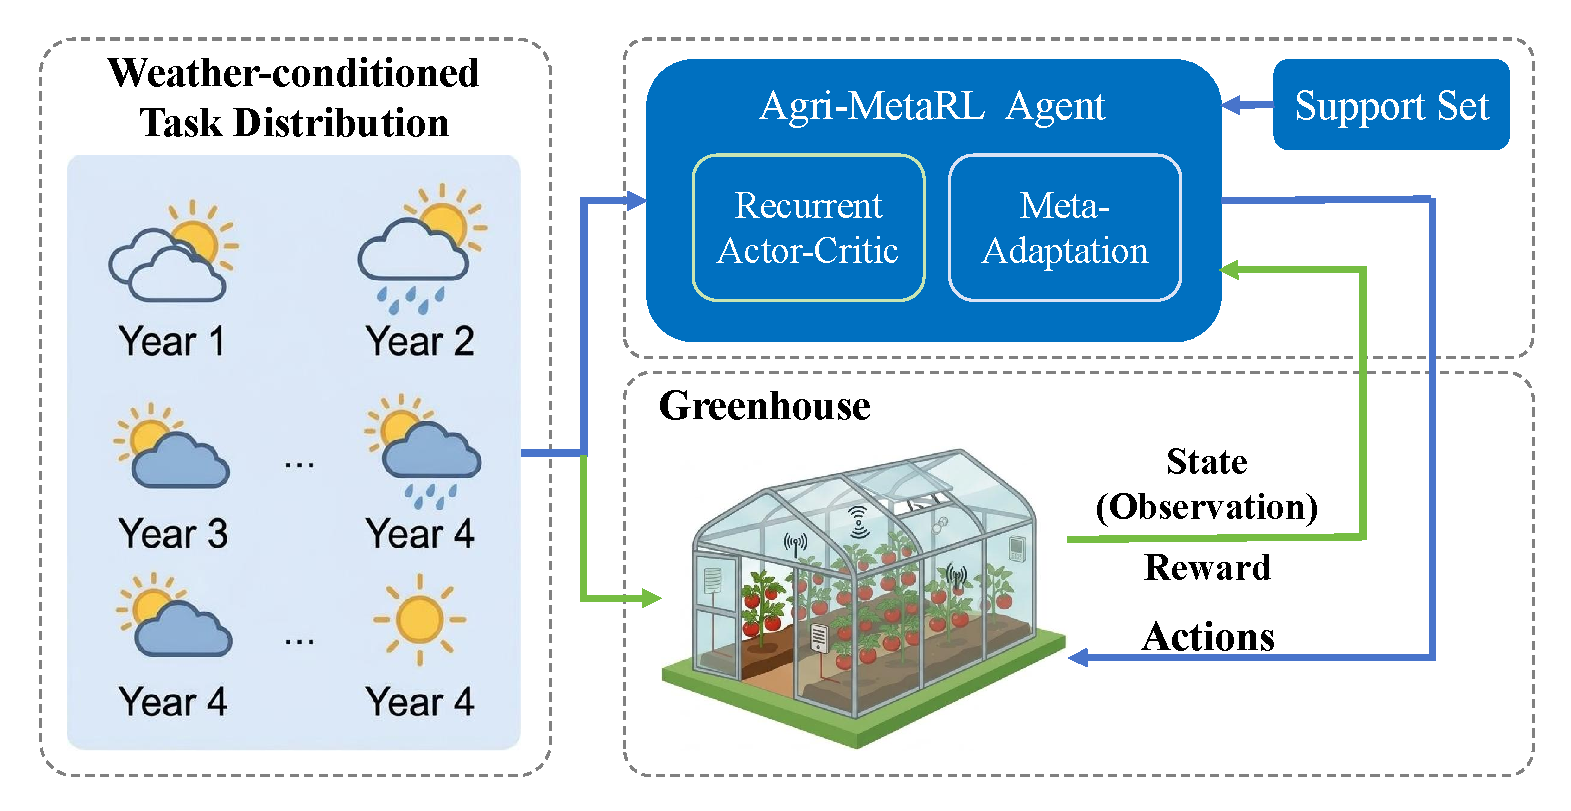
\includegraphics[width=0.9\textwidth]{visual/Figure_1.pdf}
\caption{Overall architecture of the greenhouse meta-reinforcement learning control system (Venlo-type greenhouse, tomato, GreenLight-Gym environment), including task distribution, greenhouse environment, Agri-MetaRL agent, and control variables such as temperature, humidity, and CO$_2$.}
\label{fig:system_architecture}
\end{figure}

\subsection{Base Policy: Recurrent PPO}
Agri-MetaRL uses Recurrent PPO as the base learner. PPO constrains policy update magnitude through a clipped objective~\cite{schulman2015trpo,schulman2017proximal}. GAE provides a low-variance, stable approximation for advantage estimation~\cite{schulman2015high}. Recurrent PPO further introduces LSTM to handle partial observability and temporal dependencies~\cite{ni2022recurrent,recurrentppo,hausknecht2015drqn,pleines2022recurrent}. This paper adopts a separated actor-critic LSTM structure. Both the policy and value networks use 1-layer, 256 hidden-unit LSTMs. The policy head fully connected layers are $[1024,1024]$. The value head is $[128,128]$. The learning rate is $1.161\times10^{-4}$, $\gamma=0.9631$, GAE $\lambda=0.9666$, batch size is 512, and training epochs are 8. These hyperparameters align with the GreenLight-Gym benchmark and sb3-contrib Recurrent PPO defaults~\cite{morcego2023reinforcement,van2025greenlight}, with minor adjustments from preliminary grid search to ensure comparability with baseline methods.

\subsection{Agri-MetaRL: Support-Query Advantage Correction}
Unlike typical Meta-RL methods, MAML~\cite{finn2017maml} learns a quickly adaptable initialization through inner-outer optimization loops. PEARL~\cite{rakelly2019pearl} conditions the policy on latent context variables. Both require extra gradient computation or context inference modules, and policy structure can vary with task. This paper adopts a different design. On the basis of Recurrent PPO, only the advantage estimation step is corrected in a task-aware manner during training. The policy network $\pi_{\theta}$ remains single and does not switch with task. Meta-learning is embodied in how the advantage signal used for policy gradients is adjusted according to support-derived task context. This design does not require MAML-style inner update loops. It also does not inject context into policy input like PEARL. Instead, support-query partitioning conditions the auxiliary advantage correction module. In this way, the method aims to improve cross-task generalization while maintaining training-flow compatibility with standard PPO and engineering simplicity. The unique contribution of this paper is the introduction of a support-query structure into the advantage estimation step of RL. Through the lightweight MetaAdvantageHead, the method learns how to correct advantages rather than adding task-specific policy branches.

Unlike traditional PPO and Recurrent PPO, which use the same GAE-style advantages for policy updates on all data, Agri-MetaRL splits each task segment into support and query sets. The support set encodes task context associated with the task variables $\tau=\{w,s,p,c\}$, including weather trajectory, start date, and greenhouse or scenario settings. On the query set, task-relevant correction is applied to the raw advantages. The corrected advantage $\tilde{A}_t = A_t + \delta_{\phi}(o_t, A_t, c_{\tau})$ is then used for policy updates. In this way, the training signal can vary with task context. PPO and Recurrent PPO tend to learn fixed policies on single or nearly single environment distributions. Performance may therefore degrade when task conditions change across weather years, start dates, or related settings. Agri-MetaRL instead models greenhouse control as a task distribution and learns a support-conditioned advantage correction rule during training. This design is intended to improve cross-task robustness without modifying the PPO backbone, adding extra policy branches, or introducing heavy inner-outer optimizers.

Figure~\ref{fig:meta_advantage_workflow} illustrates the workflow of the MetaAdvantageHead-based advantage correction mechanism. It contains three modules.

\begin{figure}[H]
\centering
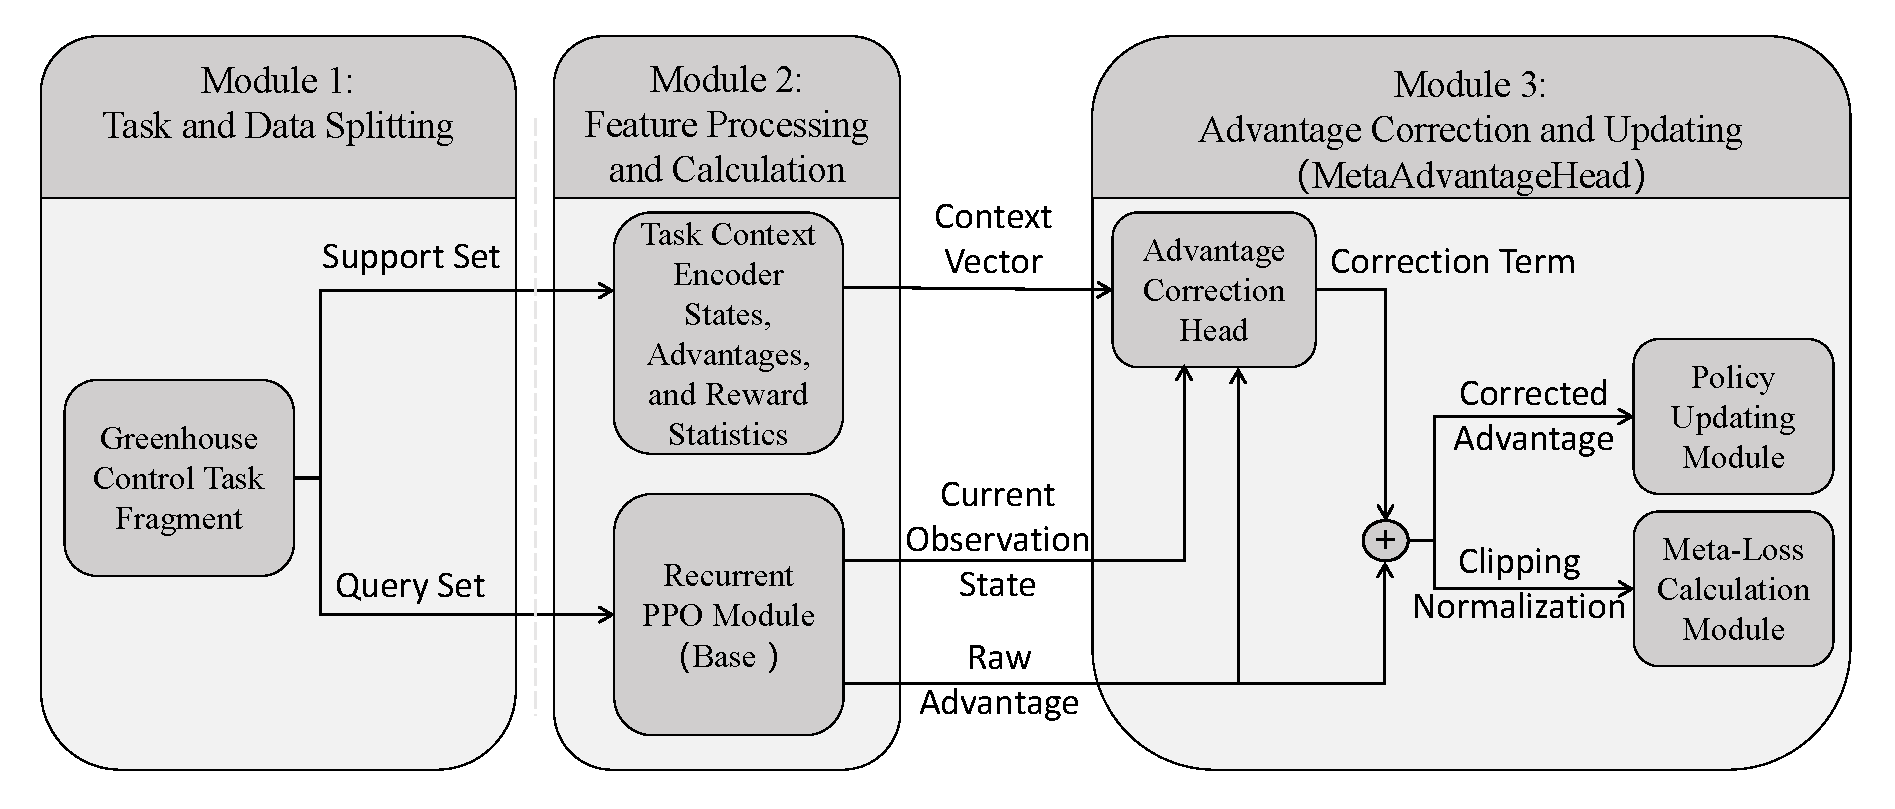
\includegraphics[width=0.95\textwidth]{visual/Figure_2.pdf}
\caption{Workflow of MetaAdvantageHead in Agri-MetaRL (based on Recurrent PPO), including task and data partitioning, feature processing and computation, and advantage correction and update modules.}
\label{fig:meta_advantage_workflow}
\end{figure}

First, each collected task segment is partitioned into support and query parts. The support set ratio is 50\% ($\mathit{meta\_support\_ratio}=0.5$). The minimum support steps are 256 ($\mathit{meta\_min\_support\_steps}=256$). Conceptually, this corresponds to an early support portion and a later query portion within the segment. Then, the support set enters the task context encoder. The encoder extracts statistics (e.g., mean and variance) from support set states, advantages, rewards, and returns, and outputs a compact context vector $c_{\tau}$. Meanwhile, the query set is processed by the base Recurrent PPO module to obtain the current observation $o_t$ and raw advantage $A_t$. Next, the advantage correction head receives three inputs: context vector $c_{\tau}$, current observation $o_t$, and raw advantage $A_t$. It outputs a correction term through the learnable network $\delta_{\phi}$, which is added to the raw advantage:
\begin{equation}
\tilde{A}_t = A_t + \delta_{\phi}(o_t, A_t, c_{\tau}),
\end{equation}
Its implementation contains a context encoder and an advantage correction head. The context encoder takes a 66-dimensional input, consisting of the mean and standard deviation of the first 30 observation dimensions in the support set, together with the mean and standard deviation of support-set advantages, rewards, and returns. It is implemented as two Linear--LayerNorm--SiLU blocks with dimensions $[66 \to 128 \to 64]$, and outputs a 64-dimensional context vector $c_{\tau}$. For each query step, the current observation $o_t$ is first projected to 64 dimensions by a linear layer. This projected observation, the raw advantage $A_t$ (1 dim), and the context vector $c_{\tau}$ (64 dim) are concatenated into a 129-dimensional input to the correction head. The correction head is a 2-layer MLP, $[129 \to 128 \to 1]$, with SiLU activation in the hidden layer, and outputs a scalar correction term $\delta_{\phi}(o_t, A_t, c_{\tau})$. The corrected advantage is then normalized and clipped before being used in PPO policy updates. For meta-loss optimization, the target advantage is defined as $G_t - V_\psi(o_t)$ and standardized within the query set, so that the auxiliary module learns task-sensitive corrections toward a return-based target.
\begin{equation}
\mathcal{L}_{meta} = \frac{1}{|\mathcal{D}_{\tau}^{qry}|}\sum_{t \in \mathcal{D}_{\tau}^{qry}} (\tilde{A}_t - \hat{A}_t)^2 + \beta \|\tilde{A}_t - A_t\|_2^2,
\end{equation}
where the target advantage $\hat{A}_t$ is defined as the difference between return and value estimate. It is standardized to zero mean and unit variance within the query set:
\begin{equation}
\hat{A}_t = \frac{(G_t - V_\psi(o_t)) - \mu_{\mathcal{D}_{\tau}^{qry}}}{\sigma_{\mathcal{D}_{\tau}^{qry}} + \epsilon},
\end{equation}
$G_t = \sum_{k=0}^{T-t} \gamma^k r_{t+k}$ is the discounted return from time $t$, $V_\psi(o_t)$ is the Critic network's value estimate for the current observation, $\mu_{\mathcal{D}_{\tau}^{qry}}$ and $\sigma_{\mathcal{D}_{\tau}^{qry}}$ are the mean and standard deviation of $G_t - V_\psi(o_t)$ within the query set, and $\epsilon$ is a numerical stability constant. $\beta$ is set to 0.05. This design preserves the PPO base structure. By making the corrected advantage approach the return-based target, the auxiliary module is encouraged to learn task-sensitive corrections that are useful for training.

From a mechanistic perspective, support trajectories provide implicit information about the current task, including weather trajectory, start date, greenhouse or scenario settings, diurnal rhythm, and crop stage. The context encoder summarizes these signals from support-set states, advantages, rewards, and returns into a compact task representation $c_{\tau}$. Conditioned on $c_{\tau}$, the correction term $\delta_{\phi}(o_t, A_t, c_{\tau})$ varies across tasks, so that the raw advantage on the query set can be adjusted in a task-dependent manner. Consequently, the corrected advantage $\tilde{A}_t$ used in PPO policy gradients reflects both the base GAE signal and support-conditioned task information. Through $\mathcal{L}_{meta}$, the auxiliary module is further encouraged to move $\tilde{A}_t$ toward the return-based target $\hat{A}_t$. If the context encoder captures features that are stable across related greenhouse tasks, this mechanism can provide a more task-aware training signal and may contribute to improved robustness on held-out weather distributions, without introducing task-specific policy branches.

\subsection{Training and Testing Protocol}
Total training steps are $2\times10^6$. The number of parallel environments is 8. Model selection uses deterministic evaluation. Approximately every $2\times10^5$ steps, evaluation is run once on the evaluation environment (training distribution: year 2010, day 59). The checkpoint with the highest mean reward is selected for subsequent evaluation. This paper uses a fixed protocol for evaluation. PPO, Recurrent PPO, Agri-MetaRL, and the rule-based baseline are compared on single-episode performance in a deterministic environment. Multi-seed testing is conducted on both training weather distribution and held-out weather distribution.

\subsection{Experimental Design and Statistical Analysis}
To evaluate method robustness, each algorithm was trained and evaluated with 5 independent random seeds. Seeds were fixed from $\{42, 123, 456, 789, 1024\}$. During training, each episode's start date was randomly sampled within the task definition range. Weather year was partitioned by training/test distribution. During testing, deterministic environment and fixed start days were used to eliminate evaluation-stage randomness. Performance comparison between methods is reported as mean $\pm$ standard deviation over 5 replicates. Given the small sample size, this paper mainly performs descriptive statistics. For inferential tests, paired $t$-test or Wilcoxon signed-rank test can be used to compare return differences between methods under the same seed.

\subsection{Evaluation Metrics}
This paper mainly uses the following metrics for evaluation: episode total return, temperature/humidity/CO$_2$ violation steps, cumulative economic metrics (Revenue, Heat, Electricity, CO$_2$, EPI), and train-vs-test distribution comparison. To analyze control behavior, this paper also presents indoor climate evolution and key actuator trajectories over the full 60 d cycle.

\subsection{Software and Reproducibility}
Experiments used Python 3.11, Stable-Baselines3, sb3-contrib, PyTorch, and GreenLight-Gym~\cite{sb3,recurrentppo,van2025greenlight,brockman2016gym,paszke2019pytorch,taksen2024gymnasium}. Unlike studies that only use off-the-shelf software and hardware, this paper implements a custom MetaAdvantageHead module on top of Recurrent PPO. This module is a researcher-developed algorithm component. It is not included in the standard implementation of Stable-Baselines3 or sb3-contrib. To support paper reproduction, this paper further provides a unified pipeline for figure and table generation, enabling reproducible generation of the figures and data summaries reported in the manuscript.

\section{Results}
\subsection{Learning Curves and Final Returns}
Figure~\ref{fig:learning_curves} shows the mean training learning curves of PPO, Recurrent PPO, and Agri-MetaRL under 5 random seeds. The shaded area indicates one standard deviation across seeds.

\begin{figure}[H]
    \centering
    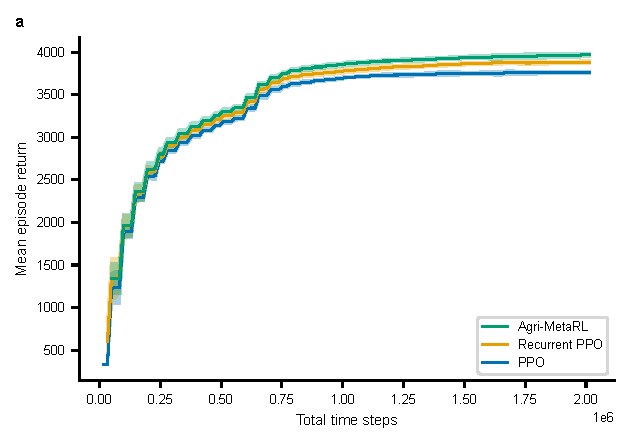
\includegraphics[width=0.8\textwidth]{visual/Figure_3.pdf}
    \caption{Episode mean return versus training steps for PPO, Recurrent PPO, and Agri-MetaRL under 5 random seeds in the GreenLight-Gym greenhouse environment; shaded area indicates mean $\pm$ standard deviation across seeds.}
    \label{fig:learning_curves}
\end{figure}

Agri-MetaRL maintains a lead from the early-mid training phase. Recurrent PPO is consistently higher than PPO overall. Table~\ref{tab:primary_results} summarizes the final mean returns. Agri-MetaRL reaches 3955 $\pm$ 16. This is higher than Recurrent PPO's 3886 $\pm$ 32 and PPO's 3811 $\pm$ 8. These results suggest that support-query advantage correction improves final performance and is associated with stable behavior across random seeds.

\begin{table}[H]
\centering
\caption{Comparison of final mean training returns under 5 random seeds}
\label{tab:primary_results}
\begin{tabular}{lc}
\toprule
Method & Final mean episode return \\
\midrule
Agri-MetaRL & $3955 \pm 16$ \\
Recurrent PPO & $3886 \pm 32$ \\
PPO & $3811 \pm 8$ \\
\bottomrule
\end{tabular}
\end{table}

\subsection{Climate Constraint Performance}
Table~\ref{tab:climate_results} compares climate violation steps of different methods under the fixed protocol.

\begin{table}[H]
\centering
\caption{Comparison of climate violation steps under fixed protocol (mean$\pm$SD; unit: steps, 15 min/step)}
\label{tab:climate_results}
\begin{tabular}{lccc}
\toprule
Method & Temperature & Humidity & CO$_2$ \\
\midrule
Agri-MetaRL & $97 \pm 44$ & $98 \pm 29$ & $11 \pm 5$ \\
Recurrent PPO & $110 \pm 55$ & $166 \pm 33$ & $28 \pm 8$ \\
PPO & $118 \pm 28$ & $172 \pm 68$ & $33 \pm 12$ \\
\bottomrule
\end{tabular}
\end{table}

Agri-MetaRL performs best on all three dimensions: temperature, humidity, and CO$_2$. Violation steps are $97 \pm 44$, $98 \pm 29$, and $11 \pm 5$, respectively. Recurrent PPO is second with $110 \pm 55$, $166 \pm 33$, and $28 \pm 8$. PPO has $118 \pm 28$, $172 \pm 68$, and $33 \pm 12$. Overall, Agri-MetaRL has a clear advantage in climate constraint control.

\subsection{Economic Metrics Comparison}
Figure~\ref{fig:economic_results} shows the cumulative economic metrics results.

\begin{figure}[H]
    \centering
    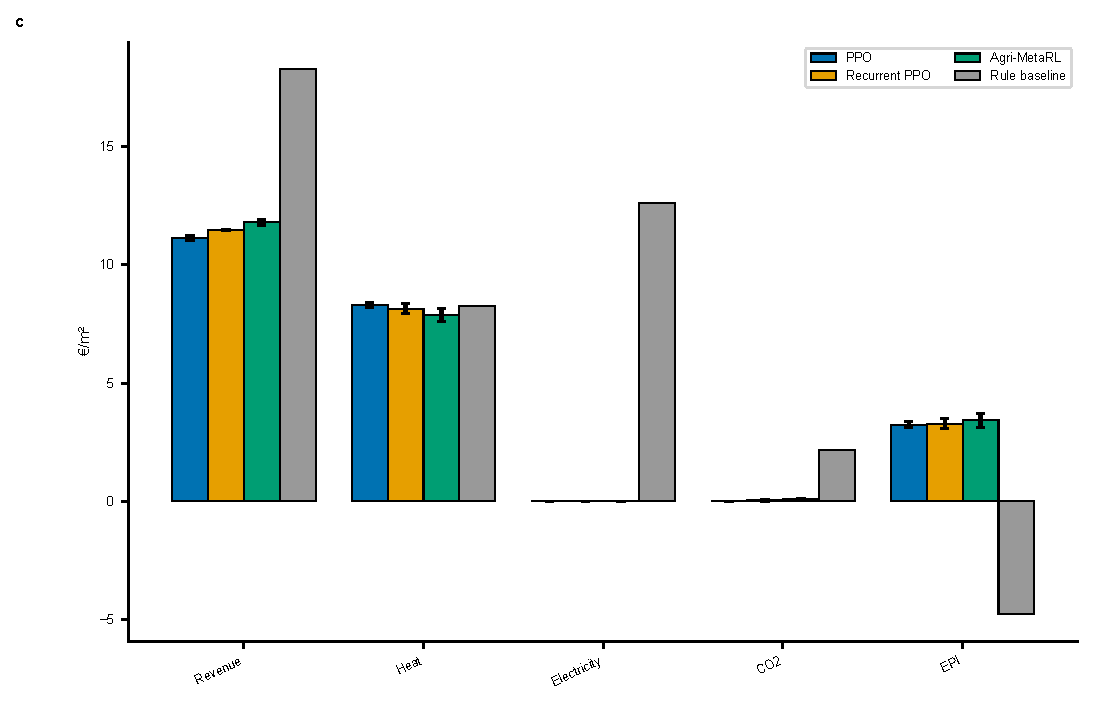
\includegraphics[width=0.88\textwidth]{visual/Figure_4.pdf}
    \caption{Comparison of cumulative economic metrics (Revenue, Heat, Electricity, CO$_2$, EPI; unit: €/m$^2$) for PPO, Recurrent PPO, Agri-MetaRL, and rule-based baseline under fixed protocol (year 2010, day 59).}
    \label{fig:economic_results}
\end{figure}

Compared with the rule-based baseline, all three RL methods significantly reduce electricity and CO$_2$ costs and improve overall economic returns. Under multi-seed statistics, Agri-MetaRL has Revenue of $11.56 \pm 0.12$ €/m$^2$, Heat of $8.12 \pm 0.32$ €/m$^2$, CO$_2$ cost of $0.08 \pm 0.02$ €/m$^2$, and final EPI of $3.46 \pm 0.30$ €/m$^2$. This is higher than Recurrent PPO's $3.34 \pm 0.22$ €/m$^2$ and PPO's $3.29 \pm 0.14$ €/m$^2$. These results suggest that support-query advantage correction can improve the balance between returns and resource consumption. The rule-based baseline has higher Revenue, but its Electricity and CO$_2$ costs are much larger. Therefore, its overall EPI remains significantly negative ($-4.76$ €/m$^2$).

Table~\ref{tab:greenlight_gym} summarizes the comprehensive performance of each controller on the training and held-out test distributions in the common GreenLight-Gym benchmark format. Return denotes episode total return. EPI is the Economic Production Index (€/m$^2$). TWB$_{\mathrm{CO}_2}$, TWB$_T$, and TWB$_{\mathrm{RH}}$ are the time-within-bounds percentages for CO$_2$, temperature, and relative humidity, respectively, converted from violation steps over the 5760-step episode. The training distribution used year 2010 weather with fixed start day (day 59). The test distribution used 2011--2013 held-out weather with start days randomly sampled from 59/80/100.

EPI and Return on the test distribution are both higher than on the training distribution. A likely reason is that the test set includes later start days such as day 80 and 100. These runs correspond to the mid-to-late growth season (approximately late March to early June), when day length is longer, heating demand is lower, and photosynthetic potential is higher. Amsterdam weather in 2011--2013 may also provide more favorable radiation and temperature conditions than 2010 in some periods. Therefore, the higher Test EPI should be interpreted mainly as a seasonal evaluation effect rather than a direct indicator of controller superiority.

\begin{table}[H]
\centering
\caption{Comprehensive performance comparison of controllers on training and held-out test distributions}
\label{tab:greenlight_gym}
\resizebox{\textwidth}{!}{
\begin{tabular}{lcccccccccc}
\toprule
& \multicolumn{5}{c}{Train ($D_{\mathrm{val}}$)} & \multicolumn{5}{c}{Test ($D_{\mathrm{test}}$)} \\
\cmidrule(lr){2-6} \cmidrule(lr){7-11}
Controller & Return & EPI & TWB$_{\mathrm{CO}_2}$ (\%) & TWB$_T$ (\%) & TWB$_{\mathrm{RH}}$ (\%) & Return & EPI & TWB$_{\mathrm{CO}_2}$ (\%) & TWB$_T$ (\%) & TWB$_{\mathrm{RH}}$ (\%) \\
\midrule
Agri-MetaRL & $3955 \pm 16$ & $3.46 \pm 0.30$ & 99.8 & 98.3 & 98.3 & $4022 \pm 83$ & 8.34 & 100.0 & 98.2 & 90.1 \\
Recurrent PPO & $3886 \pm 32$ & $3.34 \pm 0.22$ & 99.5 & 98.1 & 97.1 & $3967 \pm 77$ & 8.21 & 100.0 & 98.0 & 88.2 \\
PPO & $3811 \pm 8$ & $3.29 \pm 0.14$ & 99.4 & 98.0 & 97.0 & $3921 \pm 74$ & 8.13 & 100.0 & 97.5 & 86.3 \\
Rule-based & $3094$ & $-4.76$ & 100.0 & 92.6 & 36.2 & --- & --- & --- & --- & --- \\
\bottomrule
\end{tabular}
}
\end{table}

\subsection{60 d Full-Cycle Control Behavior Analysis}
To further observe the long-term regulation characteristics of the controller over the full growth window, Figure~\ref{fig:long_horizon_control_real} shows the actual simulation trajectories of Agri-MetaRL over the full 60 d cycle under the fixed protocol (year 2010, day 59). It includes indoor temperature, relative humidity, CO$_2$ concentration, and temporal changes in heating, ventilation, and CO$_2$ injection control signals. The climate subplots show upper and lower safety bounds. This figure was produced from recorded simulation trajectories under the fixed protocol.

\begin{figure}[H]
    \centering
    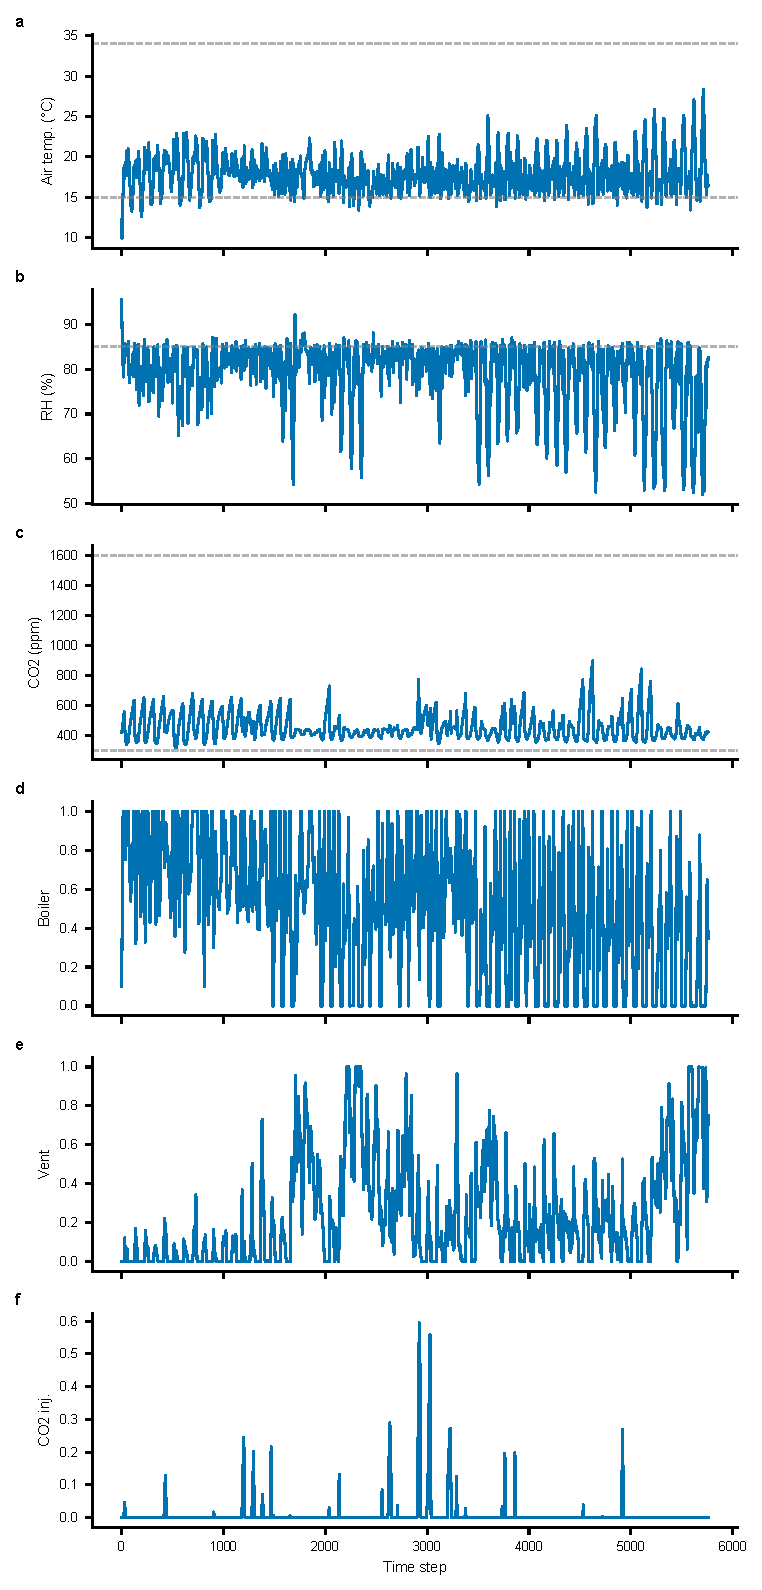
\includegraphics[width=\textwidth,height=0.88\textheight,keepaspectratio]{visual/Figure_5.pdf}
    \caption{Indoor climate variables and actuator control trajectories of Agri-MetaRL over the 60 d growth window (actual simulation results, fixed protocol year 2010 day 59). Climate variables: temperature (°C), relative humidity (\%), CO$_2$ (ppm). Control inputs: heating, ventilation, and CO$_2$ injection (dimensionless 0--1). Gray dashed lines indicate upper and lower safety bounds. Horizontal axis is time step (15 min/step).}
    \label{fig:long_horizon_control_real}
\end{figure}

The trajectories show a clear diurnal pattern over the 60 d horizon. Temperature remains within the safe range for most of the episode, with only brief night-time excursions, which is consistent with the temperature violation statistics reported in Table~\ref{tab:climate_results}. CO$_2$ concentration is generally higher during the daytime and decreases during the night, with only a small number of violations on some seeds (11 $\pm$ 5 steps in Table~\ref{tab:climate_results}). The control trajectories indicate coordinated use of heating, ventilation, and CO$_2$ injection. Heating increases during low-temperature or low-radiation periods, ventilation becomes more active under high-temperature and high-humidity conditions, and CO$_2$ injection is concentrated mainly during daytime periods when photosynthesis is active. Taken together with the learning curves, climate violation statistics, and economic metrics, these observations suggest that Agri-MetaRL maintains a balanced control behavior over the full 60 d horizon in terms of climate regulation, control smoothness, and return-oriented operation.

\section{Discussion}
The results of this paper indicate that explicitly modeling greenhouse control as a task distribution and introducing support-query advantage correction on top of Recurrent PPO merits further investigation. Compared with Recurrent PPO, Agri-MetaRL achieves higher final training return under the current protocol. It also attains the highest EPI among the RL baselines and maintains competitive performance on the held-out weather distribution. Because Return and EPI on the held-out distribution are higher than on the training distribution for all three RL methods, this pattern should be interpreted together with the seasonal differences in the evaluation protocol rather than as direct evidence of superior generalization.

Compared with existing greenhouse RL studies, Morcego et al.~\cite{morcego2023reinforcement} compared DDPG with MPC on the GreenLight model and demonstrated RL potential in greenhouse climate control. Ajagekar et al.~\cite{ajagekar2023energy} combined deep RL with robust optimization for energy-efficient control of semi-closed greenhouses. Xiao et al.~\cite{xiao2026grower} introduced a human-machine collaborative RL framework with grower participation. These studies mostly focus on single-environment or single-policy optimization. In contrast, this paper explicitly treats greenhouse control as a task distribution over weather year, start date, and scenario conditions, and introduces support-query updates during training. Under the current protocol, the resulting policy maintains competitive performance on held-out weather distributions. GreenLight-Gym~\cite{van2025greenlight} provides a standardized benchmark for greenhouse RL, and this paper further constructs a unified protocol including held-out evaluation. This facilitates comparison with subsequent studies.

From the perspective of control objective decomposition, Agri-MetaRL's main advantages are reflected in final training return and economic return (EPI). Relative to Recurrent PPO, Agri-MetaRL achieves higher return, EPI, Revenue, and better climate-constraint performance under the current protocol. In particular, final return increases from 3886 to 3955 (about 1.8\%), and EPI increases from 3.34 to 3.46 €/m$^2$ (about 3.6\%). Agri-MetaRL also records the lowest violation steps on temperature, humidity, and CO$_2$, which is consistent with the overall ranking in the learning curves and Table~\ref{tab:greenlight_gym}. These comparisons suggest that the support-query advantage correction mechanism can improve the balance between return and resource cost while preserving compatibility with the Recurrent PPO backbone and avoiding heavy inner-outer optimization. Relative to PPO, the gains are larger, but Recurrent PPO remains the primary baseline for interpreting the incremental contribution of the proposed method.

At the same time, this paper also observes clear limitations. The results are still mainly based on the current benchmark and task partitioning. Further validation of robustness is needed under richer parameter perturbations, longer time spans, and larger-scale multi-seed experiments. Future work can continue to optimize reward design, context feature construction, and multi-objective trade-offs. From a practical application perspective, Agri-MetaRL's lightweight design (no added policy branches, no heavy inner-outer optimizers) is conducive to integration into existing greenhouse control systems. The trade-off between support set length and computational cost still needs attention. In addition, simulation-to-reality transfer requires further validation in real greenhouses, especially for sensor noise, model bias, and delay.

This paper should also be viewed as an engineering prototype for Meta-RL-oriented greenhouse control, not as the final answer to the greenhouse meta-learning problem. The current implementation already has a clear support/query meta-update skeleton and a reproducible experimental and visualization workflow. But to form stronger statistical evidence, extension experiments are still needed with more seeds, richer task distributions, and more complete multi-baseline comparisons.

\section{Conclusion}
This paper proposes Agri-MetaRL, an agricultural meta-reinforcement learning algorithm for greenhouse climate control. The method formulates greenhouse control tasks as a task distribution over weather year, start date, and scenario conditions. On the basis of Recurrent PPO, it introduces the support-query MetaAdvantageHead. Support-derived task context is used to correct query advantages during training. Compared with traditional single-environment RL, Agri-MetaRL places more emphasis on a cross-task transferable update structure.

Under the current protocol, Agri-MetaRL achieved higher final training returns. It also maintained relatively stable performance on the held-out weather distribution. Climate constraint analysis and economic metrics comparison further support the effectiveness of task-context encoding and advantage correction. Overall, the results indicate that Agri-MetaRL provides a practical and extensible framework for Meta-RL-oriented greenhouse climate control research.

\section*{Declaration of Competing Interest}
The authors declare that they have no known competing financial interests or personal relationships that could have appeared to influence the work reported in this paper.

\section*{Acknowledgements}
This research was supported by [Funding Agency Name], project number [XXX].

\bibliographystyle{elsarticle-num}
\bibliography{refe}

\end{document}
